\documentclass{article}
\usepackage{graphicx}
\usepackage[utf8]{inputenc}
\usepackage[T1]{fontenc}
\usepackage{fouriernc}
\usepackage[margin=1in]{geometry}
\usepackage{amsmath}
\begin{document}

\begin{titlepage}
	\centering 
	\scshape
	\vspace*{\baselineskip}
	\rule{\textwidth}{1.6pt}\vspace*{-\baselineskip}\vspace*{2pt}
	\rule{\textwidth}{0.4pt} 
	\vspace{0.75\baselineskip}
	
	{\Large CS 374 : Computational and Numerical Methods \\\vspace{0.75\baselineskip} Assignments}
	\vspace{0.75\baselineskip}
	
	\rule{\textwidth}{0.4pt}\vspace*{-\baselineskip}\vspace{3.2pt} 
	\rule{\textwidth}{1.6pt}
	
	\vspace{2\baselineskip}  
	Computational and Numerical Method
	
	\vspace*{3\baselineskip}
	
	\vspace{0.5\baselineskip} %originally 0.5
	
	{\scshape\large Purvil Mehta (201701073) \\ Bhargey Mehta (201701074) \\} 
	
	\vspace{1\baselineskip} 
	
	\textit{Dhirubhai Ambani Institute of Information and Communication Technology \\ Gandhinagar\\} 
	\vspace*{2\baselineskip}
	\today


\end{titlepage}

\newpage
\tableofcontents
\newpage
\section{Assignment 1}
\subsection{The Entropy Function}
We have the entropy function as,
\large{$$\langle I \rangle = -k \sum p_i\log{p_i}$$}

\subsection{Plots}
\begin{figure}[!h]
    \centering
    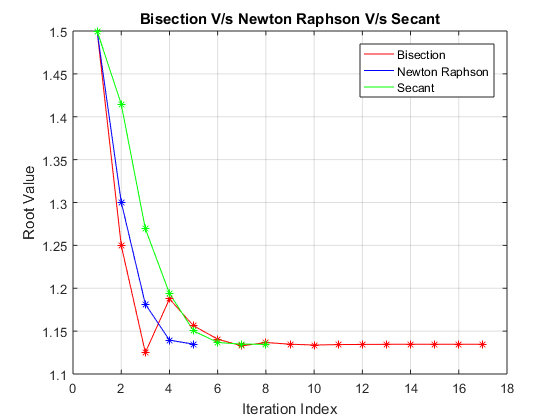
\includegraphics[scale = 0.71]{1_1.png}
    \caption{Entropy Function for k = 1}
\end{figure}

\subsubsection{Observation}
\begin{itemize}
    \item We can see that the function peaks at $p = \frac{1}{2}$
    \item We can interpret this as maximum information available at $p = \frac{1}{2}$ so the function peaks at that point. At $p = 0$ or $p = 1$, we already know what event is going to take place so the information we obtain from that event is 0.
\end{itemize}

\subsubsection{Equations}
\begin{equation*}
  \begin{aligned}
    \langle I \rangle &= -k[p\log_2{p} + (1-p)\log_2{(1-p)}]\\
    \frac{\mathrm{d}}{\mathrm{d}p}\langle I \rangle &= -k[\log_2{p} + 1 + -\log_2{(1-p)} -1]/ln(2) = 0\\
  \end{aligned}
\end{equation*}
So we have,
\begin{equation*}
  \begin{aligned}
     -k[\log_2{p}  -\log_2{(1-p)} ]/ln(2) = 0\\
     \log_2{p} = \log_2{(1-p)}\\
     p = 1 - p\\
     p = \frac{1}{2}
  \end{aligned}
\end{equation*}

\subsection{Approximation}
Apply a very small perturbation as $p = \frac{1}{2} + \epsilon$, in which $\epsilon << \frac{1}{2}$. Show that in this perturbation
approach $\langle I \rangle \approx a - b\epsilon^2$, with $a = k$ and $b = \frac{4k}{\ln2}$.
\newline
We will be using the approximation $\ln{(1+x)} \approx x$
\newline
\newline
We have

\begin{equation*}
  \begin{aligned}
    \langle I \rangle &= -k[p\log_2{p} + (1-p)\log_2{(1-p)}]\\
    &= -k[(\frac{1}{2} + \epsilon)\log_2{(\frac{1}{2} + \epsilon)} + (\frac{1}{2} - \epsilon)\log_2{(\frac{1}{2} - \epsilon)}]\\
    &= -k[\frac{1}{2}(\log_2{(\frac{1}{2} + \epsilon)} + \log_2{(\frac{1}{2} - \epsilon)}) + \epsilon (\log_2{(\frac{1}{2} + \epsilon)} - \log_2{(\frac{1}{2} - \epsilon)})]\\
    &= -\frac{k}{\ln2}[\frac{1}{2}(\ln{(\frac{1}{2} + \epsilon)} + \ln{(\frac{1}{2} - \epsilon)}) + \epsilon (\ln{(\frac{1}{2} + \epsilon)} - \ln{(\frac{1}{2} - \epsilon)})]\\
    &= -\frac{k}{\ln2}[\frac{1}{2}(\ln{(\frac{1+2\epsilon}{2})} + \ln{(\frac{1-2\epsilon}{2})}) + \epsilon (\ln{(\frac{1+2\epsilon}{2})} - \ln{(\frac{1-2\epsilon}{2})})]\\
    &= -\frac{k}{\ln2}[\frac{1}{2}(\ln{(1+2\epsilon)} + \ln{(1-2\epsilon)} - 2\ln2) + \epsilon (\ln{(1+2\epsilon)} - \ln{(1-2\epsilon)} + \ln2-\ln2)]\\
    &\approx -\frac{k}{\ln2}[\frac{1}{2}(2\epsilon -2\epsilon - 2\ln2) + \epsilon (2\epsilon - (-2\epsilon))]\\
    &\approx -\frac{k}{\ln2}[\frac{1}{2}(-2\ln2) + \epsilon (4\epsilon)]\\
    &\approx -\frac{k}{\ln2}[-\ln2 + 4\epsilon^2]\\
    &\approx k-(\frac{4k}{\ln2})\epsilon^2\\
  \end{aligned}
\end{equation*}
\newline
\newline
Thus we have $\langle I \rangle \approx k-(\frac{4k}{\ln2})\epsilon^2$ with $a = k$ and $b = \frac{4k}{\ln2}$ by comparison.

\newpage
\subsection{Plots}
$$\langle I \rangle = -k[p\log_2{p} + (1-p)\log_2{(1-p)}]$$
$$\langle I \rangle \approx k-(\frac{4k}{\ln2})\epsilon^2$$
\begin{center} where $p = \frac{1}{2} + \epsilon$ \end{center}

\begin{figure}[!h]
    \centering
    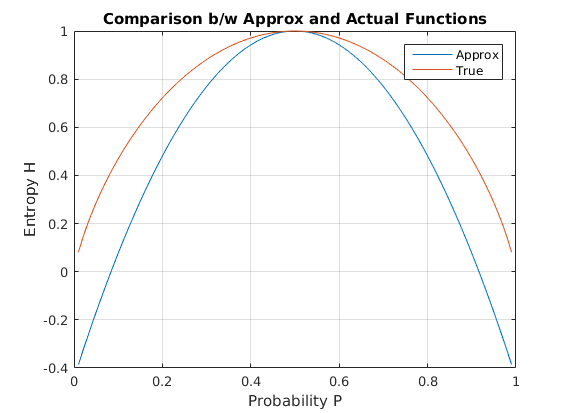
\includegraphics[scale=0.8]{1_2.png}
    \caption{Actual Function V/s Approximation}
\end{figure}
\newpage

\section{Assignment 2}
\subsection{Plots}
\begin{figure}[!h]
    \centering
    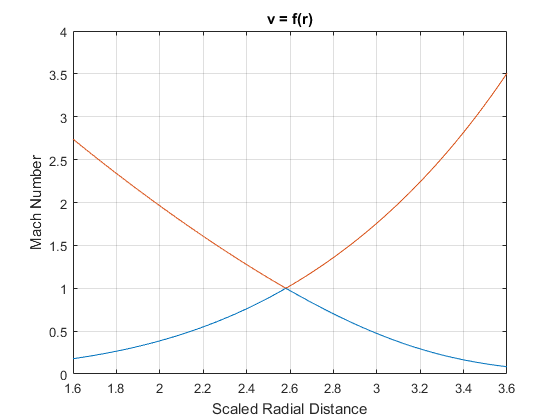
\includegraphics[scale = 0.8]{2_1.png}
    \caption{Two plots corresponding to $v = f(r)$}
\end{figure}
\begin{figure}[!h]
    \centering
    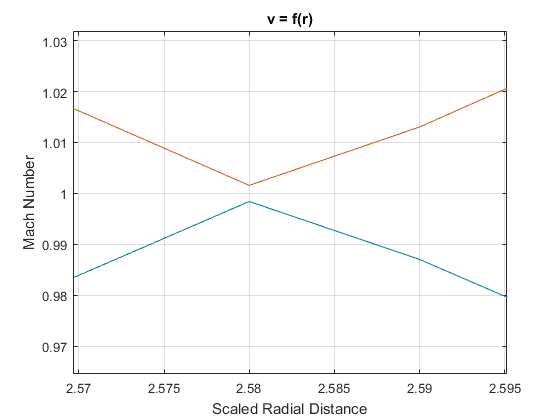
\includegraphics[scale = 0.8]{2_2.png}
    \caption{The Plots don't meet but they do come close}
\end{figure}

\newpage
\subsection{Code Run-time}
\begin{figure}[!h]
    \centering
    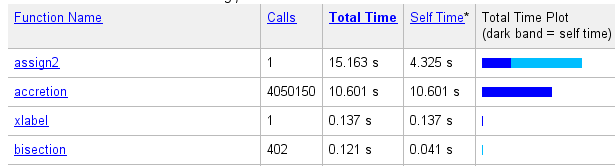
\includegraphics[scale = 0.9]{2_time_1.png}
    \caption{$\triangle V = 10$}
\end{figure}
\begin{figure}[!h]
    \centering
    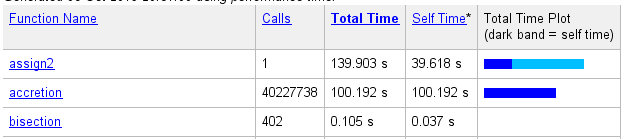
\includegraphics[scale = 0.9]{2_time_2.png}
    \caption{$\triangle V = 1$}
\end{figure}
\begin{figure}[!h]
    \centering
    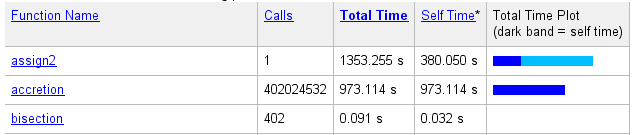
\includegraphics[scale = 0.9]{2_time_3.png}
    \caption{$\triangle V = 0.1$}
\end{figure}    
\newpage

\section{Assignment 3}
\begin{figure}[!h]
    \centering
    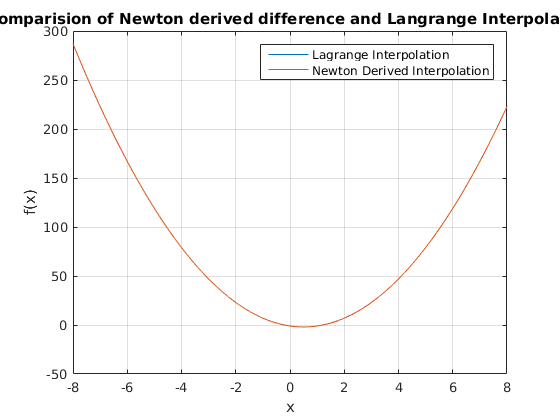
\includegraphics[scale = 1]{3_1.png}
    \caption{$y = y(R), u = u(R)$}
\end{figure}
\subsection{Analytical Methods}
$$xyR^2 = 1$$
$$y^4 - By^2 - \frac{4y}{R^2} + \frac{3}{R^4} = 0$$
$$\frac{dy}{dR} = \frac{2(3 - 2yR^2)}{R^3(2y^3R^2 - ByR^2-2)}$$
\par The turning point in the velocity profile occurs when the
numerator in the RHS becomes zero. Hence we have $y = \frac{3}{2R^2}$, which gives us $x = \frac{2}{3}$.

Solution for the y will be
$$y = - \frac{-R^4 + 4R^2 + \sqrt{(R^4 - 4r^2)^2 + 12R^4B}}{2R^4B}$$
$$y = - \frac{-R^4 + 4R^2 - \sqrt{(R^4 - 4r^2)^2 + 12R^4B}}{2R^4B}$$
\newpage

\section{Assignment 4}
\begin{figure}[!h]
    \centering
    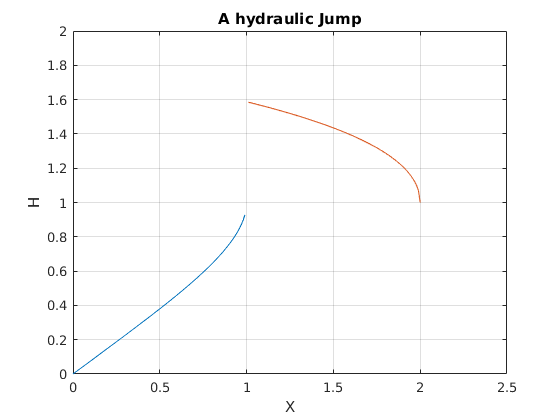
\includegraphics[scale = 1]{4_1.png}
    \caption{$H = H(X)$}
\end{figure}
\subsection{Analytical Methods}
$$4H - H^4 = 3(X - D)$$
$$\frac{dH}{dX} = \frac{3}{4(1 - H^3)}$$

By looking at the above equation we can say that at $H = 1$ slope of the function become $\infty$. Thus at point $H = 1$ ,function will take hydraulic jump and will be discontinuous.  
\newpage
\section{Assignment 5}

\begin{figure}[h!]
    \centering
    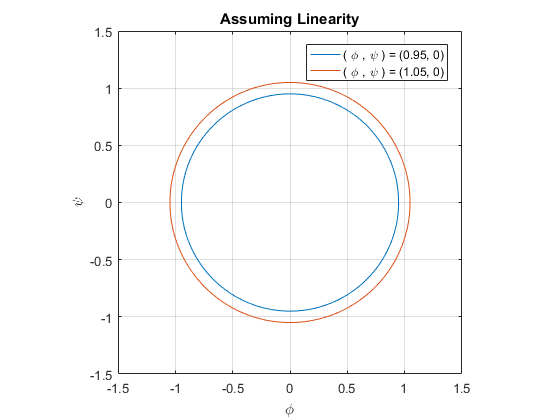
\includegraphics[scale = 0.6]{ass5_1.png}
    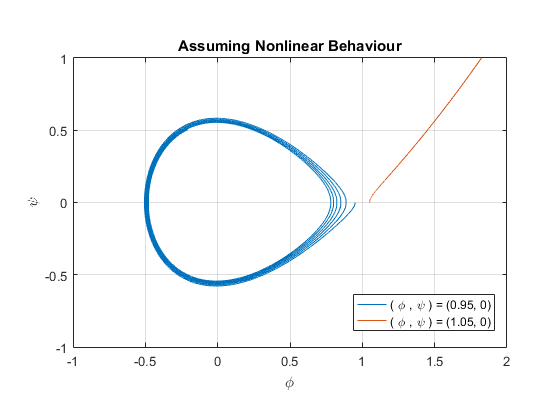
\includegraphics[scale = 0.6]{ass5_2.png}
    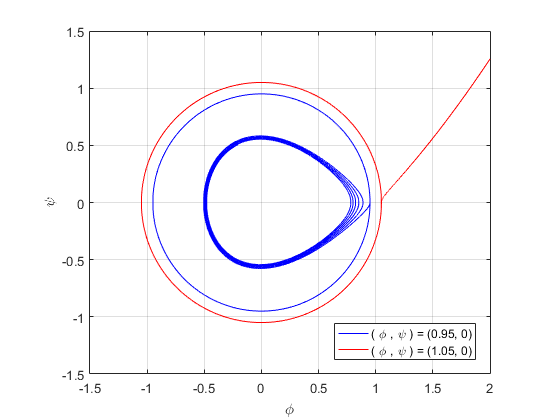
\includegraphics[scale = 0.6]{ass5_3.png}
\end{figure}


\end{document}